\documentclass[tikz,border=8pt]{standalone}
\usepackage{fontspec}
\usepackage{amsmath}
\usetikzlibrary{arrows.meta,calc,decorations.markings}

\setmainfont{Arial}
\setsansfont{Arial}

\definecolor{fieldblue}{HTML}{12AEEA}
\definecolor{lineblack}{HTML}{111827}
\definecolor{textmain}{HTML}{0F172A}

\begin{document}
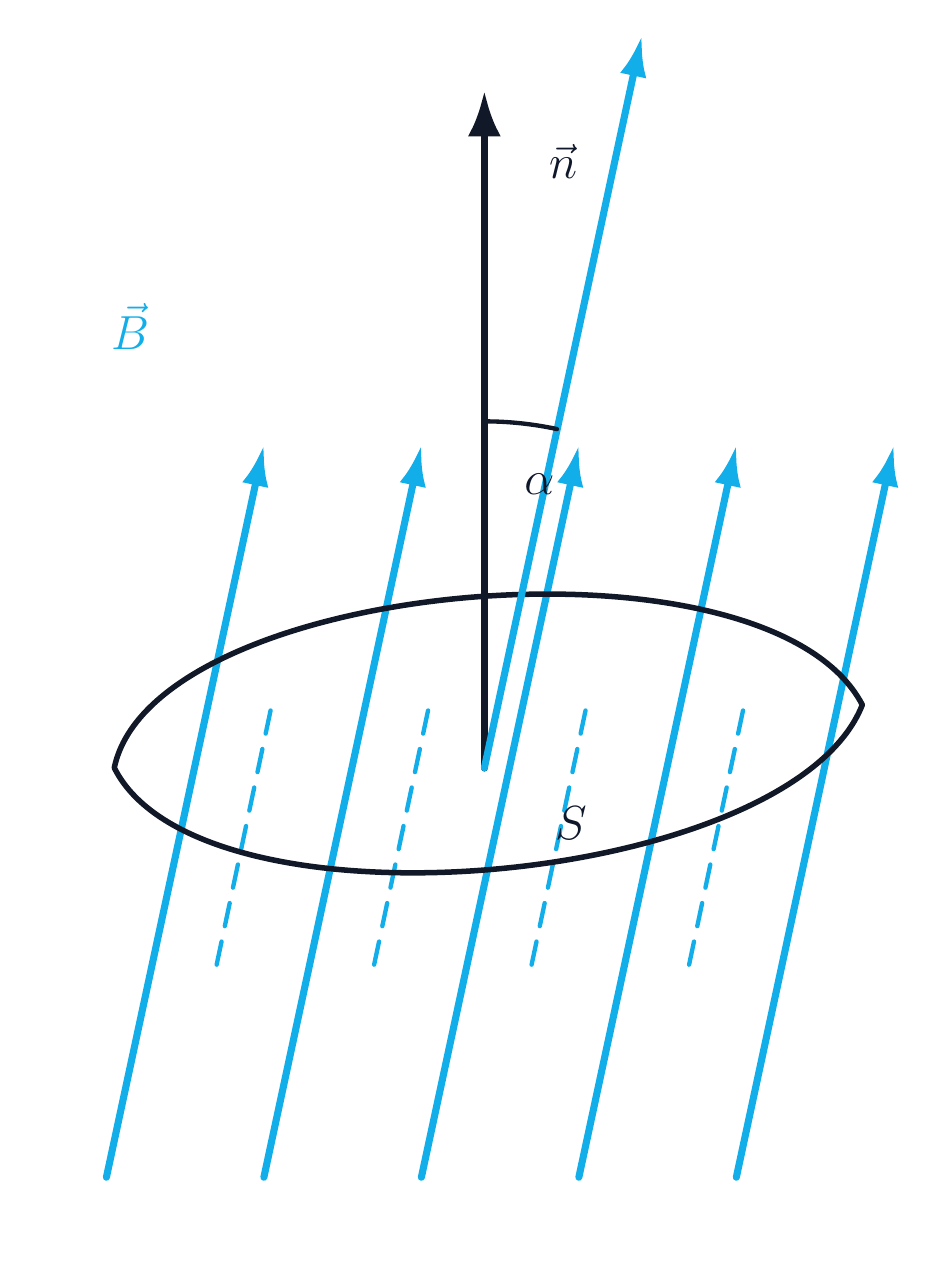
\begin{tikzpicture}[
  x=1mm,y=1mm,line cap=round,line join=round,
  font=\sffamily,
  fieldline/.style={fieldblue,line width=0.9mm,-{Latex[length=5.2mm,width=3.4mm]}},
  hiddenfield/.style={fieldblue,line width=0.55mm,dashed,dash pattern=on 3mm off 2mm},
  normal/.style={lineblack,line width=0.95mm,-{Latex[length=5.8mm,width=4.2mm]}},
  angle/.style={lineblack,line width=0.55mm}
]
  \fill[white] (-6,-10) rectangle (104,144);

  % Magnetic induction lines, tilted like the reference image.
  \foreach \x in {4,24,44,64,84} {
    \draw[fieldline] (\x,-2) -- ++(20,93);
  }
  \foreach \x in {18,38,58,78} {
    \draw[hiddenfield] (\x,25) -- ++(7,33);
  }

  % Surface crossed by the magnetic field.
  \draw[lineblack,line width=0.7mm] (5,50)
    .. controls (10,74) and (88,81) .. (100,58)
    .. controls (91,35) and (16,28) .. (5,50);

  % Central normal and reference field direction from the same point.
  \coordinate (O) at (52,50);
  \draw[normal] (O) -- (52,136);
  \draw[fieldline] (O) -- ++(20,93);

  % Angle between n and B.
  \draw[angle] (52,94) arc[start angle=90,end angle=77.9,radius=44];
  \node[font=\sffamily\itshape\fontsize{17}{20}\selectfont,text=textmain] at (59,86) {$\alpha$};

  % Labels.
  \node[font=\sffamily\itshape\fontsize{17}{20}\selectfont,text=fieldblue] at (7,106) {$\vec B$};
  \node[font=\sffamily\itshape\fontsize{16}{19}\selectfont,text=textmain] at (62,127) {$\vec n$};
  \node[font=\sffamily\itshape\fontsize{17}{20}\selectfont,text=textmain] at (63,43) {$S$};
\end{tikzpicture}
\end{document}
